\section{Variable Selection}
\label{sec:variable_selection}

Since the total number of numerical covariates is 47, we perform a variable selection procedure to identify the most relevant predictors $X_{ij}^*$ for the response $y_i^*$.\\

In a preliminary step, we drop specific variables deemed irrelevant by the sociological literature, most of which are related to the territorial characteristics of the provinces. Specifically, we drop: \texttt{urban\_type}, \texttt{area\_km2}, \texttt{internet\_coverage\_rate}, \texttt{green\_m2\_capita}, \texttt{eco\_urban\_index}.

Subsequently, we remove variables with a Pearson or Spearman's correlation coefficient $|\rho_{ij}| \ge 0.85$ with women's employment rate, such as \texttt{empl\_rate}, \texttt{unempl\_rate}, \texttt{inact\_rate}, \texttt{young\_neet}, \texttt{fem\_house\_rate}, \texttt{part\_rate}. Since the women's employment rate is the proportion of working women in working age, over all women of working age, all the aforementioned variables partially contain the same information, thus resulting in extremely high correlation coefficients.\\

Additionally, within each group of covariates (ECEC and non-ECEC), pairs of highly correlated variables are identified. For any pair with an absolute Pearson correlation coefficient $|\rho_{ij}| \ge 0.80$, one variable is discarded to mitigate multicollinearity. During this process, multiple variables are removed from the non-ECEC subset, such as \texttt{male\_edu\_rate}, dropped in favour of \texttt{fem\_edu\_rate}, \texttt{fertility\_rate} and \texttt{dependency\_rate}, which are dropped in favour of \texttt{ageing\_index}; finally, \texttt{GDP}, \texttt{foreign\_rate}, \texttt{adj\_net\_migration\_rate}, \texttt{n\_large\_comp}, and \texttt{house\_price} are removed, while \texttt{graduate\_mobility\_rate} is kept. Among the ECEC variables, we find that \texttt{other\_per\_capita\_expenditure} is virtually equal to \texttt{other\_percapita\_public\_expenditure}  ($|\rho_{ij}| = 0.99$). Additionally, \texttt{ecec\_participation} is highly correlated with both \texttt{per\_capita\_public\_expenditure} and \texttt{per\_capita\_user\_contribution}, which are highly correlated among themselves. Finally, \texttt{coverage} and \texttt{private\_coverage} show a high correlation, motivated by design, since $coverage_i = public\_coverage_i + private\_coverage_i$. For these reasons, we remove from our analysis the following ECEC variables: \texttt{coverage}, \texttt{per\_capita\_public\_expenditure}, \texttt{per\_capita\_user\_contribution} and \texttt{other\_per\_capita\_expenditure}.\\

After evaluating the variance inflation factor of the remaining variables, we note that most values are above 2, and some above 5\footnote{The table of VIF values can be inspected in Appendix A, table \ref{tab:vif_values}}.  We decide to apply a Bayesian Lasso approach \citep{Park2008} to perform further shrinkage and variable selection. The corresponding model specification, the distributions of $\beta_j$ coefficients (Figure \ref{fig:bayesian_lasso_results}) and the variables selected (Table \ref{tab:variable_selection_table}) are reported below:\\

\begin{align*}
    y^{\ast}_i \mid \boldsymbol{\beta}, \sigma, \phi_i 
        &\stackrel{\text{ind}}{\sim}\mathcal{N}\big(\alpha + \phi_i +  \boldsymbol{x}_i^{\ast \top} \boldsymbol{\beta},\, \sigma^2\big) \, ,
        \quad i = 1,\dots,N \\
    \beta_j \mid \lambda, \sigma 
        &\stackrel{\text{iid}}{\sim}\mathrm{Laplace}\big(0,\, \sigma / \lambda\big) \, ,
        \quad j = 1,\dots,P \\
    \lambda^2 &\sim \mathrm{Gamma}(2, 1), \\
    \sigma &\sim \mathrm{HalfNormal}(1), \\
    \alpha &\sim \mathcal{N}\big(0, \, 10^2),\\
    \phi \mid \tau_c, \rho, W &\sim \mathcal{N}_N \big(\boldsymbol{0},[\tau_c (D -\rho W)]^{-1} \big)\, \\
    \rho &\sim \mathrm{Beta}(2,2),\\
    \tau_c &\sim \mathrm{Gamma}(1,1).
\end{align*}\\

The Laplace prior can be expressed as a scale mixture of normals, leading to strong shrinkage of small coefficients toward zero while allowing relevant predictors to retain non-negligible effects. The global shrinkage parameter 
$\lambda$ controls the overall degree of penalization and is assigned a Gamma prior.\\

In addition, to account for residual spatial dependence in the response, we include a spatial random effect $\boldsymbol{\phi}$, modeled through a proper conditional autoregressive (CAR) prior. The structure matrix $(D - \rho W)$ is defined by the adjacency matrix $W$ of the areal units and the corresponding diagonal matrix $D$, where $D_{ii}$ equals the number of neighbors of province $i$. The parameter $\rho$ controls the strength of spatial autocorrelation, while $\tau_c$ governs the overall precision of the spatial effect. Weakly informative priors are adopted for $\alpha$ and $\sigma$, while $\rho$ and $\tau_c$ are assigned Beta and Gamma priors, respectively.\\

This formulation allows variable selection to be performed while simultaneously accounting for spatially structured unobserved heterogeneity, reducing the risk of selecting spurious covariates due to spatial autocorrelation in the residuals. The selection criteria adopted is to keep covariates that didn't include 0 in their 95\% CI.

\begin{table}[h]
    \centering
    \begin{tabular}{cc}
        \hline
        \textbf{ECEC variables} &  \textbf{Non-ECEC variables}\\
        \hline
        \texttt{private\_coverage} & \texttt{fem\_maj\_empl\_rate}\\
        \texttt{public\_coverage} & \texttt{service\_empl\_rate}\\
        \texttt{} & \texttt{graduate\_mobility\_rate}\\
        \texttt{} & \texttt{empl\_growth}\\
        
        \hline
    \end{tabular}
    \caption{Selected variables for the model.}
    \label{tab:variable_selection_table}
\end{table}

\begin{figure}[h]
    \centering
    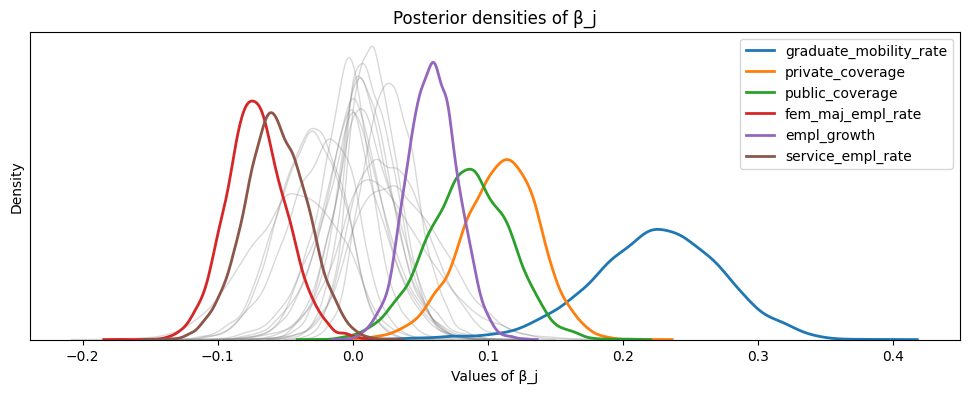
\includegraphics[width=0.9\linewidth]{chapters/images/final_variable_selection.png}
    \caption{Posterior densities of the coefficients $\beta_j$ and selected variables.}
    \label{fig:bayesian_lasso_results}
\end{figure}
